\cchapter{کارهای مرتبط}
\label{related-works}

در این قسمت به بیان کارهای انجام شده در این حوزه خواهیم پرداخت و برای این کار درخت موضوعی مرتبط با آن رسم شده. هر گره ار درخت موضوعی یک راهکار برای جلوگیری از رخداد شروع سرد است و هر گره دارای بخش‌هایی است تا به برگ برسیم. در شکل \ref{fig:subject-tree} درخت موضوعی نمایش داده شده است و هر گره را به ترتیب بررسی خواهیم کرد. 

\begin{figure}
	\centering
	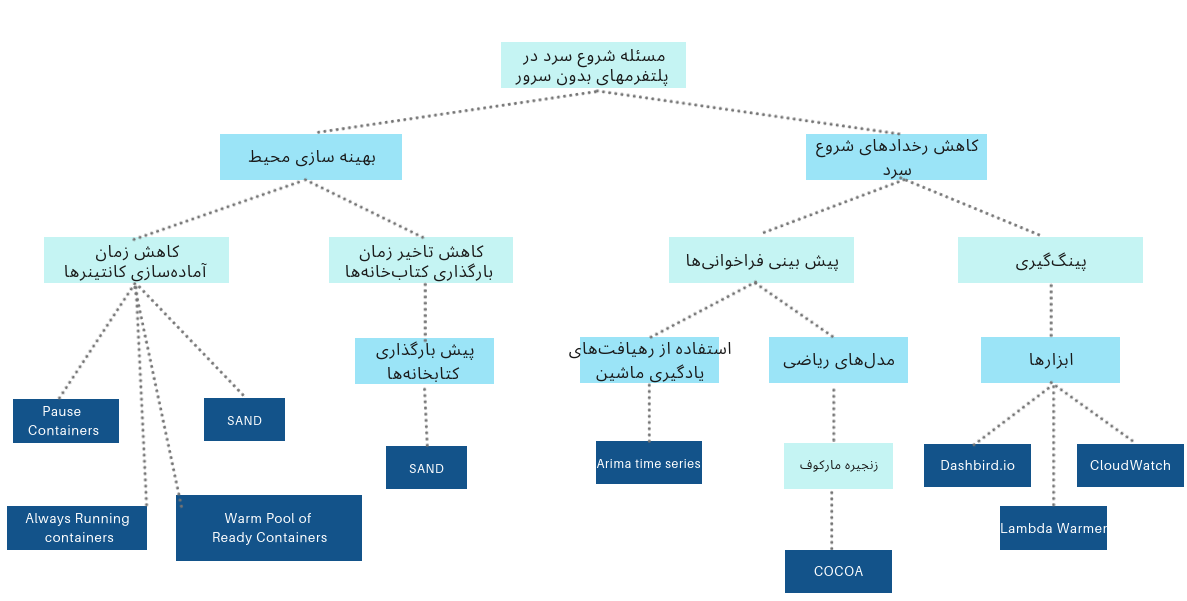
\includegraphics[width=\linewidth]{figs/subject-tree}
	\caption {درخت موضوعی}
	\label{fig:subject-tree}
\end{figure}

ریشه درخت مسئله شروع سرد است که ۲ گره اصلی دارد. گره سمت چپ که بهینه سازی محیط نام دارد، تلاش می‌کند تا در صورت وجود رخداد شروع سرد زمان آن‌را به حداقل برساند. این گره ۲ فرزند دارد که عبارتند از کاهش تاخیر آماده سازی کانتینرها و کاهش زمان بارگذاری کتابخانه‌ها. یک روش برای کاهش زمان بارگذاری کتاب‌خانه ها استفاده از روش پیش-بارگذاری است. 


گره سمت راست ریشه هم کاهش رخداد‌های شروع سرد است. تمرکز این گره در این است نگذاریم شروع سرد رخ دهد. گره سمت راست این نود، روش پینگ‌گیری است؛ در این روش سعی می‌کنیم با استفاده از ابزارهایی جلوگیری کنیم از سرد شدن توابع. در آخرین سطح این گره هم ابزارهای مرتبط معرفی شده‌اند. فرزند سمت چپ گره کاهش رخداد، پیش‌بینی فراخوانی‌ها است. در پیش‌بینی فراخوانی ها می‌توان از رهیافت‌های بدست آمده در یادگیری ماشین بهره جست. روش دیگر استفاده از مدل‌های ریاضیاتی غیریادگیری ماشین برای پیش‌بینی فراخوانی‌ها است. یکی از این روش‌های استفاده از ماشین‌ّهای حالت محدود بدست آمده با روش‌زنجیره مارکوف است.

 
در برگ‌های این درخت هرکدام یک مقاله را بررسی می‌کنیم. در ابتدا به توضیح درباره روش‌های بهینه‌سازی محیط می‌پردازیم و سپس به سراغ کاهش رخداد میرویم. در هر حوزه یک مقاله نمونه بررسی خواهد شد. 

\section{ بهینه سازی محیط}
          
          در این روش قرار به این است که مانع وقوع شروع سرد نشویم (در واقع هم نمی‌توان مانع از اتفاق شروع سرد شد)؛ بنابران به دنبال روش‌ یا روش‌هایی برای کاهش زمان شروع سرد هستیم. همانگونه که بالاتر ذکر کردیم، این موضوع را می‌توان از دو جنبه بررسی کرد. اول اینکه آماده‌سازی کانتینر‌ها را کاهش دهیم. روش دیگر این است که زمان لودشدن کتابخانه‌ها برای اجرای تابع را کاهش دهیم. برای این کار می‌شود از روش پیش-بارگذاری کتابخانه ها استفاده کرد.  
          
\subsection{کاهش زمان آماده‌سازی کانتینرها}

در این روش دنبال کمینه‌سازی زمان شروع سرد با استفاده از روش‌هایی برای کانفیگ بهینه محیط برای مواجهه با شروع سرد هستیم. عمده کارهایی که در این بخش انجام می‌دهیم در سطح شبکه یا کانتینر‌ها برای بهینه سازی است که روش‌های نسبتا سطح پایینی محسوب می‌شوند. 

یکی از مواردی که شروع سرد به شدت رخ می‌دهد، زمانی است که بنابه‌دلایلی تابع درخواست‌های زیادی دارد. این موضوع در \cite{lin2019mitigating} ذکر شده است. نویسنده معتقد با انجام این بهبودها در حدود 85٪ مدت‌زمان شروع سرد برای این توابع صرفه‌جویی خواهد شد. این مقاله از پلتفرم \lr{Knative} برای پیاده‌سازی تغییرات استفاده می‌کند. علت انتخاب \lr{Knative} این است که بر روی بستر کوبرنتیز ساخته می‌شود و از مفاهیمی مثل \lr{Pod} ها برای اجرای توابع و جریان‌های کاری استفاده می‌کند. بنابراین، از آنجایی که کوبرنتیز دست ما را برای انجام تغییرات باز می‌گذارد، می‌توان به آسانی به پیاده سازی سیاست‌های\LTRfootnote{policy} خودمان بپردازیم. در پلتفرم \lr{Knative} هر تابع در درون یک پاد اجرا می‌شود. پادها، ابتدایی‌ترین و ساده‌ترین بارهای‌کاری (به هر برنامه درحال اجرا در کوبرنتیز بارهای کاری می‌گوییم. توجه داشته باشید در کوبرنتیز بارکاری یک موجودیت نیست در واقع مفهومی است که به اجرای کانتینر‌ها و تخصیص \lr{CPU} و … اشاره دارد.) در کوبرنتیز هستند. در درون هر پاد تعدادی کانتینر اجرا می‌شود. در یک پاد شبکه‌ها، ذخیره سازی (Storage)‌ به صورت مشترک است. البته باز هم به خاطر وجود بحث‌هایی مثل \lr{Cgroups} و \lr{namespace} که ساختمان داده اصلی کانتینرها هستند، کانتینرهای داخل یک پاد از هم ایزوله هستند. پادهادر کوبرنتیز موجودیت‌های موقتی هستند و درصورت از دست رفتن نود، اتمام کار، کمبود منابع سرور و دلایل دیگر می‌توانند از سرور خارج شوند و دیگر قابل بازیابی نیستند. 

نکته‌ای که باید توجه داشت این است که یک پاد از جنس یک پردازه\LTRfootnote{Process} نیست؛ بلکه، محیطی منطقی برای اجرای کانتینر‌هاست و این کانتینرها هستند که از جنس پردازه‌ها هستند. داده‌های درون کانتینر‌ها وابسته به پادها هستند و با ری‌استارت شدن پادها محتویات ذخیره شده در کانتینرها از بین می‌روند مگر اینکه در ذخیره‌سازها ذخیره بشوند.\cite{KubernetesInAction}

با توجه به مقدماتی که در مورد پاد‌ها ذکر شد، اکنون منطقی به نظر می‌رسد برای مدیریت کانتینر‌ها بخواهیم از پادها استفاده کنیم و این رهیافت دست ما را برای اعمال تغییرات مختلف روی پلتفرم باز می‌کند. 

ما به صورت ایده‌آل دنبال کمترین سربار برای فراخوانی توابع هستیم. هنگامی که برای اولین بار تابع را فراخوانی می‌کنیم دچار تاخیر شروع سرد می‌شویم که در بخش ادبیات موضوع (رفرنس به شروع سرد)‌ در مورد آن مفصلا بحث کردیم. این مشکل در تمامی پلتفرم‌های بدون سرور، مشکل رایجی است. سربار شروع سرد را می‌توان به ۲ قسمت تعیین کرد :‌

\begin{enumerate}
	\item سربار ناشی از اجرای پلتفرم
	
علت اصلی این سربار اجرای پلتفرم است و به علت قرار گرفتن در صف یا دلایل دیگر باعث تاخیر می‌شود. از این دسته خطا‌ها می‌توان به network bootstraping، pod provisioning یا nework sidecar اشاره کرد. 
	
	\item سربار ناشی از خود اپلیکیشن
	
علت اصلی این سربار مشکلات خود برنامه است. این نوع تاخیر به مواردی از جمله زبان برنامه‌نویسی، حجم برنامه و نوع کتاب‌خانه‌هایی که از آن‌ها استفاده می‌کنیم بستگی دارد.
	
	
\end{enumerate}
 

برای مثال اجرای یک \lr{HTTP Server} ساده شروع سردی در حدود 5 ثانیه را به خود اختصاص می‌دهد؛ درحالی‌که با اجرای یک برنامه کلاس‌بندی عکس زمان شروع سرد به چیزی در حدود 40 ثانیه هم برسد. 

بنابراین، ایده این مقاله این است که برای اجرای توابعی که اخیرا محبوب شد‌ه‌اند از رهیافت استفاده از یک استخر گرم برای نگه‌داری این پاد استفاده‌کنیم. دقت کنید که در اینجا، در داخل هر پاد تنها یک کانتینر که آن کانتینر هم برای یک تابع است، اجرا می‌شود. هرگاه که درخواست جدید برای تابع می‌رسد در ابتدا استخر گرم را چک می‌کنیم که آیا پاد در آن موجود است یا خیر؟ اگر پاد در آن وجود داشت دیگر منتظر نمی‌مانیم، سریع تابع را در پلتفرم اجرا کرده و دیگر تاخیر شروع سرد را نخواهیم داشت. بنا به محاسبه نویسنده مقاله، این روش تا 85٪ زمان شروع سرد را برای توابع \lr{on-demand} نسبت به حالت عادی، کاهش می‌دهد. 

اما چگونه این تغییرات انجام شده است؟ شکل \ref{fig:knative-architecturea} نمایشگر معماری پلتفرم بدون سرور \lr{Knative} است. انتظار داریم با بهینه‌سازی‌هایی این رهیافت را برای مدیریت شروع‌های سرد اعمال کنیم. 

\begin{figure}
	\centering
	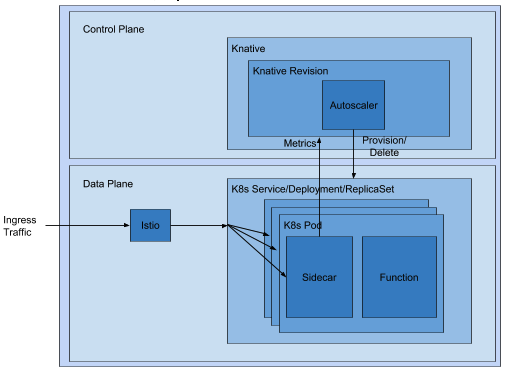
\includegraphics[width=\linewidth]{figs/knative-architecture}
	\caption {معماری پلتفرم Knative}
	\label{fig:knative-architecture}
\end{figure}

همانگونه که در این شکل می‌بینیم، وظیفه مولفه \lr{autoscaler}،  انجام وظایف مربوط به \lr{Scale up/down} است. هنگامی که دچار شروع سرد می‌شویم، مولفه \lr{autoscaler} دستور به ساخت پاد را می‌دهد  ولی از آنجایی که این امر وقت گیر است انجام آن بسیار طول می‌کشد. نهایتا اینکه پس از مدت زیادی پاد ساخته شده و داخل بخش \lr{data plane} اجرا می‌شود.

برای حل این مشکل، مقاله پیشنهاد می‌دهد تا در بخش \lr{control plane} و داخل \lr{revision} پلتفرم \lr{knative} یک مولفه مدیریت استخر قرار دهیم که آن با توجه به درخواست‌هایی که برای \lr{auto-scaler} می‌رسد، اقدام به ساخت پاد‌هایی و نگه‌داری آن در استخر گرم که در بخش \lr{data plane} توسعه داده شده، می‌کند. استخر گرم محدودیت ‌هایی مثل اندازه استخر دارد و تنها تعداد محدودی پاد در آن می‌توان نگه داشت.  حال اگر درخواستی برای پلتفرم برسد، \lr{autoscaler} ابتدا از کنترل کننده استخر\LTRfootnote{pool controller} وضعیت موجودی در استخر گرم را بررسی می‌کند. اگر در استخر پاد موجود باشد در اینصورت بلافاصله مهاجرت(migration)  از استخر گرم به سرویس رخ می‌دهد. از آنجایی که در استخر گرم منابع به پاد اختصاص داده شده و پاد کاملا آماده‌ی اجرا است؛ بنابراین، تاخیر شروع سرد بسیار ناچیزی خواهیم داشت. اما از طرفی، اگر پاد در استخر گرم موجود نباشد، دچار تاخیر شروع سرد خواهیم شد. نکته‌ی منفی این روش این است که در صورت رخداد شروع سرد، به میزان تاخیر‌های قبل، تاخیر ناشی از استعلام از استخر گرم ‌هم اضافه خواهد شد. شکل \ref{fig:Knative-architecture-modified} مدل جدید مقاله برای مدیریت شروع سرد را نشان می‌دهد. \cite{KubernetesInAction} 

\begin{figure}
	\centering
	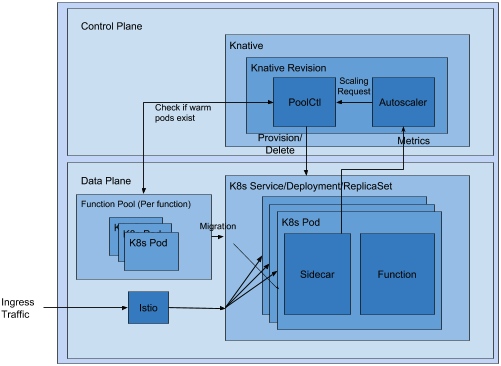
\includegraphics[width=\linewidth]{figs/Knative-architecture-modified}
	\caption {معماری پیشنهادی مقاله برای حل تاخیر شروع سرد}
	\label{fig:Knative-architecture-modified}
\end{figure}

\par
\par
مقاله دیگری که در این حوزه اقدام به بررسی تاثیر آماده سازی کانتیرها پرداخته از ایده pause container ها که مفهومی در کوبرنتیز است استفاده می‌کند. \ref{mohan2019agile}
این مقاله اقدام به بررسی تاخیر شروع سرد ناشی از اجرای همزمان تعدادی تابع کرد و نتایج خروجی آن را در شکل \ref{fig:coldstart-importance} نشان داده‌اند. 

در این واقع، این مقاله تاخیر شروع سرد را ناشی از آماده سازی کانتینر‌ها می‌بیند و سعی می‌کند تا حد امکان با آن مقابله کند. برای نمایش و پیاده‌سازی سناریو خود از پلتفرم‌ \lr{Apache OpenWhisk} استفاده کرده‌اند. طبق همان شکل نتیجه می‌گیریم که بخش عمده‌ای از تاخیرها ناشی از تاخیر در آماده‌سازی کانتینرها است، زیرا باید گام‌های طولانی برای ساخت و استقرار یک کانتینر و اختصاص شبکه به آن برداریم. شکل \ref{fig:container-network-creation} این گام ها را نشان می‌دهد.

\begin{figure}
	\centering
	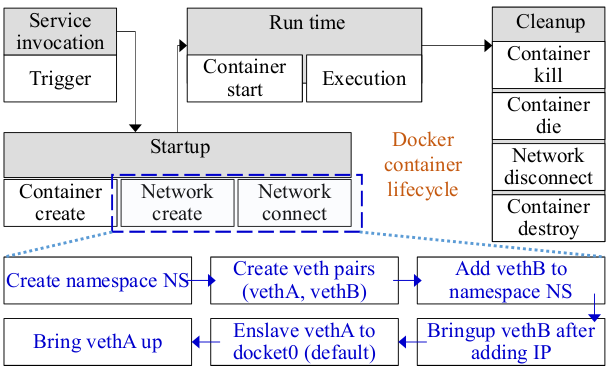
\includegraphics[width=\linewidth]{figs/container-network-creation}
	\caption {مراحل ساخت یک فضای نام در داکر}
	\label{fig:container-network-creation}
\end{figure}

همانگونه که در شکل مشخص است برای اجرای یک تابع در پلتفرم، ابتدا باید کانتیر آن ساخته شود. بسیاری از پلتفرم‌ها از جمله پلتفرم \lr{OpenWhisk} - که این مقاله تغییرات را بر بستر این پلتفرم بدون سرور انجام می‌دهد، - ازموتور داکر به عنوان موتنو کانتینری در پلتفرم خود پشتیبانی می‌کنند. در این موتور مراحل شکل فوق باید انجام بشود تا یک کانتینر کاملا آماده شود.

با توجه به شکل، تمامی بهبودهایی که باید انجام دهیم در مرحله شروع اولیه کانتینر است، جایی که دقیقا 3 مرحله داریم. ساخت کانتینرها، ساخت شبکه‌ها و اتصال کانتینرها به آن‌ها و در نهایت اتصال شبکه‌ها. 

در مرحله‌ای اول باید فضای نام‌را برای هر شبکه ایجاد کنیم. این کار در داکر توسط یک ویژگی کرنل لینوکس به نام فضای نام \LTRfootnote{namespace} انجام می‌گیرد. فضای نام یه مانع یا ایزوله کننده شبکه است که فرایند مختلف را از یکدیگر جدا می‌کند. در هر فضای نام پس از ایزوله سازی می‌توان مطمئن بود که دسترسی به پردازه‌های دیگر به شدت محدود شده است. اما، ما به دنبال ایزوله کردن پروسه نیستیم، بلکه به دنبال این هستیم که اجرا پردازه در سیستم عامل ایزوله باشد ولی ارتباط با آن نیز ممکن باشد. بنابراین باید تنظیمات شبکه در آن را انجام دهیم. 

بنابراین به دنبال ایجاد جفت‌های \lr{veth} \LTRfootnote{namespace} هستیم. جفت‌های \lr{veth} یک سری کابل مجازی هستند ( به طور دقیق از جنس خط لوله‌ها در سیستم عامل هستند) که وظیفه انتقال یک طرفه از کانتینر به فضای بیرون از آن و بالعکس را دارا می‌باشند. پس اقدام به اضافه کردن \lr{veth}ها به شبکه می‌کنیم. این دوقسمتی که مطرح شد خود شامل 6 مرحله کلی می‌شود که توضیح آن در این گزارش جایی ندارد.

حال نقش شبکه‌ها در شروع سرد چیست؟‌ همانگونه که قبلا گفتیم، هر کانتینر از 4 مرحله می‌گذرد. مرحله اول، مرحله فراخوانی سرویس هاست که در آن یک درخواست ساخت کانتینر برای \lr{docker daemon} ارسال می‌شود. مرحله دوم مرحله آغاز‌کردن\LTRfootnote{Startup} نام دارد که در طی آن یک کانتینر باید برای اتصال به محیط پیرامون آماده شود بنابراین کانتینر ساخته شده، شبکه درون و بیرون کانتینر کانفیگ می‌شود و به هم متصل می‌شوند.. مرحله سوم مرحله اجرا\LTRfootnote{execution} است که در طی آن، تابع اجرا می‌شود و در انتها مرحله‌ی نهایی یا مرحله پاکسازی\LTRfootnote{Cleanup} را داریم که شامل توقف اجرای کانتینر، قطع اتصال شبکه و نابود سازی آن است. 

علاوه ساخت کانتینرها،‌ به این توجه کنید که ما به دنبال اجرای همزمان آن‌ها نیز هستیم. این مورد زمان و سربار اجرا را نیز به طرز قابل توجهی بالا می‌برد.	اگر به شکل \ref{fig:coldstart-importance} نگاه کنید مجددا می‌بینید که به ازای اجرا‌های همزمان، زمان آماده‌سازی بسیار طولانی‌تر شده است درحالی‌که، زمان اجرا تغییر چندانی نکرده است. 

مقاله می‌گوید که بر طبق آمارهای گرفته شده، در مرحله آماده‌سازی کانتینرها، 90٪ زمان آماده‌سازی مربوط به ۲ مرحله ساخت شبکه‌ها و اتصال شبکه‌ها می‌شود. بنابراین معتقد است که با بهبود در این وضعیت تاخیر شروع سرد تا حد قابل توجهی برای تمامی توابع، کاهش خواهد یافت. حال مشکل اینجا‌است که این مراحل به کندی انجام می‌شوند مثلا برای ساخت شبکه این کار یکی یکی و در یک صف به نوبت انجام می‌شود. با توجه به اینکه در پلتفرم‌های بزرگ و تجاری در هر لحظه تعداد زیادی کانتینر باید ساخته یا حذف شوند این تاخیر به شدت افزایش پیدا خواهد کرد. برای اینکار آزمایشی انجام شد که نتایج آن در جدول \ref{table:1} قابل مشاهده است. 
\par

\begin{table}[h]
	\begin{center}
		\caption{زمان ساخت و پاکسازی کانتیرهای همزمان}
		\begin{tabular} {| c | c | c | c | c |}
			\hline
			
			تعداد فضا‌های نام همزمان & $1$ & $10$ & $50$ & $100$ \\
			\hline
			زمان ساخت & $0.28$ & $1.27$ & $6.28$ & $14.41$ \\
			\hline
			زمان پاکسازی & $0.20$ & $0.71$ & $3.24$ & $7.77$ \\
			\hline
		\end{tabular}
	\label{table:1}
	\end{center}
\end{table}

همانگونه که در این جدول قابل مشاهده است، زمان آماده‌سازی سرویس‌ها به ازای تعداد تعداد کانتینرهای همزمان، به طور نمایی افزایش می‌یابد. در حالی‌که ما در پلتفرم‌های تجاری همزمان تعداد زیادی کانتینر را هم بسازیم یا از بین ببریم. 

بهتر است به این دید نگاه کنیم که \lr{pause container} ها از قبل شبکه را ساخته و کانفیگ‌های مربوطه را انجام داده‌اند. پس کانتینری که در درون آن اجرا می‌شود تنها به معرفی برای اختصاص آدرس IP دارند که کار زمان‌بری نیست. بنابراین، می‌توان پس از ساخت یک کانتینر، تنها به اجرای آن در \lr{pause container} ها بپردازیم و از این طریق در زمان ساخت بسیار صرفه جویی کنیم. همچنین برای پاکسازی تنها باید کانتینر تابع مربوطه را حذف کنیم و \lr{pause container} بازیابی می‌شود. این رهیافت در شکل \ref{fig:pause-container-solution} نشان داده شده است.

\begin{figure}
	\centering
	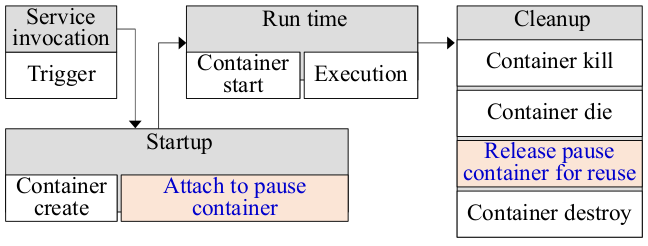
\includegraphics[width=\linewidth]{figs/pause-container-solution}
	\caption {استفاده از \lr{Pause Container}ها برای کاهش تاخیر شروع سرد}
	\label{fig:pause-container-solution}
\end{figure}

در این حالت دو مرحله ساخت و اتصال شبکه جایگزین شده. همچنین برای مدیریت \lr{pause container} ها نیز یک استخر مربوط به آن‌ها ساخته‌شده است. در شکل \ref{fig:Pause-Container-Pool-Manager} نحوه عملکرد این رهیافت توضیح داده شده است.

\begin{figure}
	\centering
	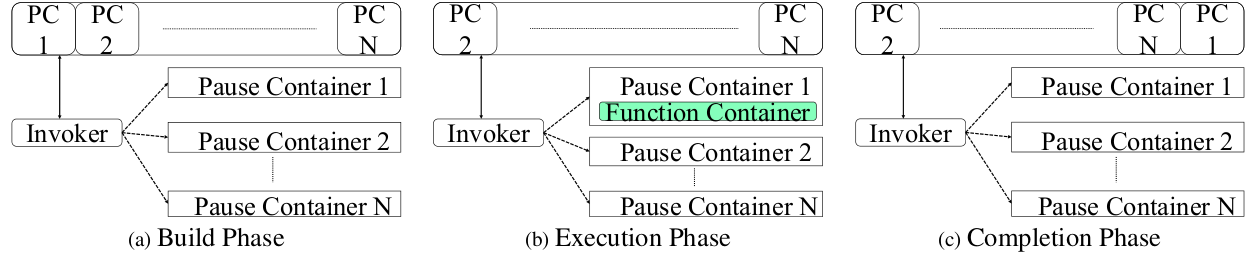
\includegraphics[width=\linewidth]{figs/Pause-Container-Pool-Manager}
	\caption {مدیر استخر \lr{Pause Container}ها}
	\label{fig:Pause-Container-Pool-Manager}
\end{figure}
 
در قسمت اول که فاز ساخت است۷ از قبل تعدادی کانتینر ساخته شده و در یک صف نگهداری می‌شوند. یک فراخواننده\LTRfootnote{invoker} داریم که وضعیت تمامی PC\LTRfootnote{مخفف Pause Container}ها را می‌داند. در قسمت بعدی می‌خواهیم یک تابع را اجرا کنیم؛ برای اینکار تنها کافی‌است که آن کانتینر را درون PC بارگذاری کنیم. و هرگاه کار تابع تمام شد تنها کافی است آن کانتینر در \lr{PC} را نابود کنیم. در انتها خود \lr{PC} بازیابی می‌شود و به انتهای صف استخرهای \lr{PC} اضافه می‌شود. 

نتایج این رهیافت در شکل زیر نشان داده شده است و می‌تواند تا 80٪ زمان شروع سرد را برای توابع کاهش دهد. برای مقایسه میزان بهبود داده شده شکل را با شکل مقایسه کنید.


\begin{figure}
	\centering
	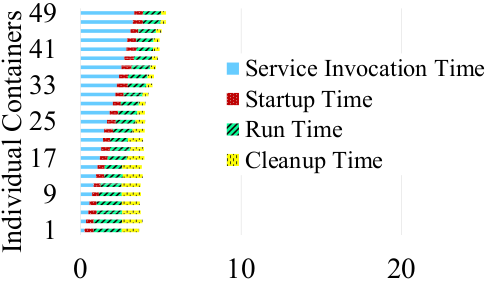
\includegraphics[width=\linewidth]{figs/Pause-Containers-Results}
	\caption {نتیاج و بهبود حاصل شده با استفاده از \lr{Pause Container}ها}
	\label{fig:Pause-Containers-Results}
\end{figure}


\section{کاهش رخداد‌های شروع سرد}

در این قسمت به دنبال روش‌هایی برای کاهش احتمال شروع سرد در پلتفرم‌های بدون سرور هستیم. در واقع ما به دنبال این هستیم که جلوی رخداد شروع سرد را با هایی بگیریم. از دسته‌بندی‌های کلی در این مبحث می‌وان به روش‌های جلوگیری از شروع سرد با استفاده از پینگ‌گیری یا روش‌های پیش‌بینی شروع سرد، اشاره کرد. 